\documentclass[a4paper]{article}

\usepackage[english]{babel}
\usepackage[utf8x]{inputenc}
\usepackage[T1]{fontenc}

\usepackage[a4paper,top=3cm,bottom=3cm,left=2cm,right=2cm,marginparwidth=1.5cm]{geometry}

\usepackage{amsfonts}
\usepackage{amsmath}
\usepackage{amssymb}
\usepackage{amsthm}
\usepackage{graphicx}
\usepackage[ruled,vlined]{algorithm2e}
\usepackage[colorinlistoftodos]{todonotes}
\usepackage[colorlinks=true, allcolors=blue]{hyperref}

\setlength\parindent{0pt}

\DeclareMathOperator*{\argmax}{argmax}
\DeclareMathOperator*{\argmin}{argmin}
\newcommand*{\vertbar}{\rule[-1ex]{0.5pt}{2.5ex}}
\newcommand*{\horzbar}{\rule[.5ex]{2.5ex}{0.5pt}}

\newtheorem{theorem}{Theorem}[section]
\newtheorem{lemma}[theorem]{Lemma}

\title{CS 395T: Homework 3}
\author{Brady Zhou \\ brady.zhou@utexas.edu}

\begin{document}

\maketitle

\section{Low Rank Matrix Recovery (Alternating Minimization)}

We are interested in minimizing the following
\begin{align*}
\argmin_{B, C} \sum_{i=1}^n \sum_{j=1}^n g_{ij} (a_{ij} - B_i^\intercal C_j)^2 + \frac{\mu}{2} (||B||_F^2 + ||C||_F^2)
\end{align*}

We can do this by taking partials with respect to row vectors $B_k^\intercal$ and column vectors $C_k$.
\begin{align*}
\frac{\partial}{\partial B_k^\intercal} \Big( \sum_{i=1}^n \sum_{j=1}^n g_{ij} (a_{ij} - B_i^\intercal C_j)^2 + \frac{\mu}{2} (||B||_F^2 + ||C||_F^2) \Big)
&= -2 \sum_{j=1}^n g_{kj} (a_{kj} - B_k^\intercal C_j) C_j^\intercal + \mu B_k^\intercal \\
\frac{\partial}{\partial C_k} \Big( \sum_{i=1}^n \sum_{j=1}^n g_{ij} (a_{ij} - B_i^\intercal C_j)^2 + \frac{\mu}{2} (||B||_F^2 + ||C||_F^2) \Big)
&= -2 \sum_{i=1}^n g_{ik} (a_{ik} - B_i^\intercal C_k) B_i + \mu C_k
\end{align*}

Setting $\frac{\partial}{\partial B_k^\intercal} = 0$, we have the following
\begin{align*}
0 &= -2 \sum_{j=1}^n g_{kj} (a_{kj} - B_k^\intercal C_j) C_j + \mu B_k^\intercal \\
2 \sum_{j=1}^n g_{kj} a_{kj} C_j^\intercal &= B_k^\intercal \Big(2 \sum_{j=1}^n g_{kj} C_j C_j^\intercal + \mu I \Big) \\
2 \sum_{j=1}^n g_{kj} a_{kj} C_j &= \Big(2 \sum_{j=1}^n g_{kj} C_j C_j^\intercal + \mu I \Big) B_k^{\intercal^\intercal} && \text{Transpose for sanity.}
\end{align*}

So we can see the optimal $B_k^\intercal$ is the solution to $Ax = b$, where 
\begin{align*}
A &= 2 \sum_{j=1}^n g_{kj} C_j C_j^\intercal + \mu I \\
b &= 2 \sum_{j=1}^n g_{kj} a_{kj} C_j
\end{align*}

Similarly, for column vectors $C_k$,
\begin{align*}
0 &= -2 \sum_{i=1}^n g_{ik} (a_{ik} - B_i^\intercal C_k) B_i + \mu C_k \\
2 \sum_{i=1}^n g_{ik} a_{ik} B_i &= \Big( 2 \sum_{i=1}^n g_{ik} B_i B_i^\intercal + \mu I \Big) C_k
\end{align*}

And we have our result.

\begin{figure}[!h]
\centering
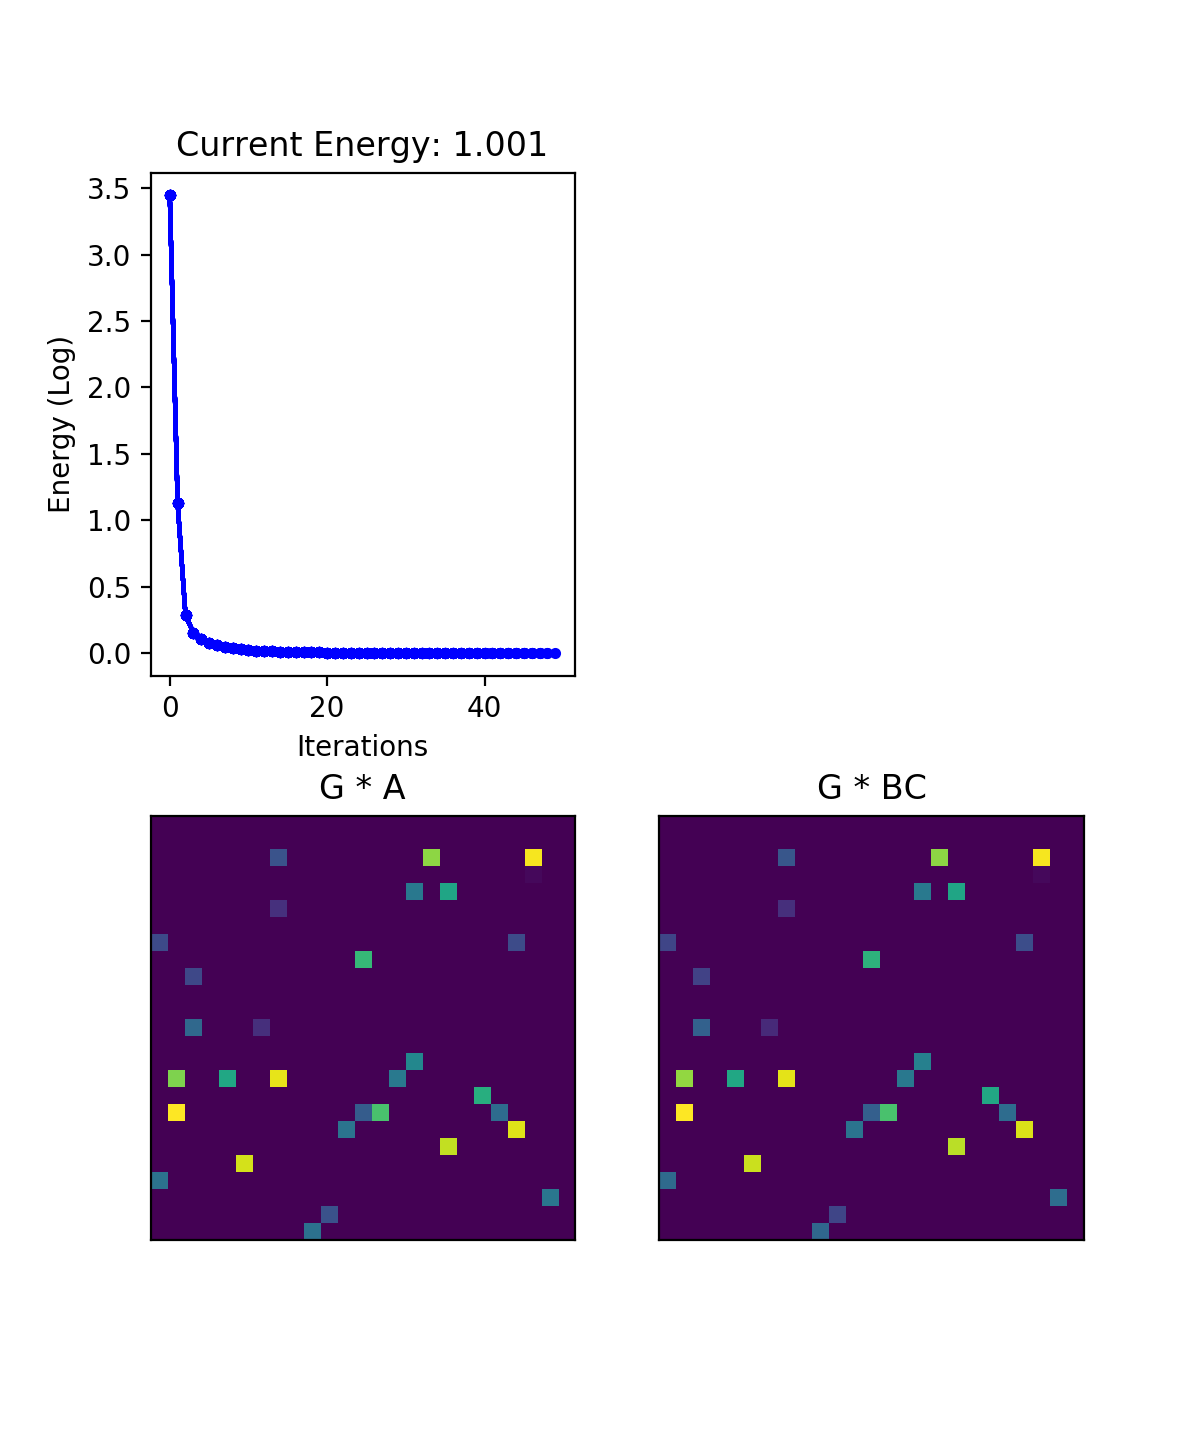
\includegraphics[width=0.5\textwidth]{low_rank_am.png}
\caption{Results of alternating minimization.}
\end{figure}


\section{Low Rank Matrix Recovery (Newton Trust Region)}

To perform the Newton Trust Region method, we will have to calculate the Hessian of the objective function, where we are now minimizing over
\begin{align*}
    x = \begin{bmatrix}
        B_1^{\intercal^\intercal} \\
        B_2^{\intercal^\intercal} \\
        \vdots \\
        B_n^{\intercal^\intercal} \\
        \horzbar \\
        C_1 \\
        C_2 \\
        \vdots \\
        C_n \\
        \end{bmatrix}
\end{align*}

Restating the result from Problem 1,
\begin{align*}
\frac{\partial f}{\partial B_i^{\intercal^\intercal}} &= -2 \sum_{k=1}^n g_{ik} (a_{ik} - B_i^\intercal C_k) C_k + \mu B_i^{\intercal^\intercal} \\
\frac{\partial f}{\partial C_i} &= -2 \sum_{k=1}^n g_{ki} (a_{ki} - B_k^\intercal C_i) B_k^{\intercal^\intercal} + \mu C_i
\end{align*}

By inspection, we can see $\frac{\partial f}{\partial B_i^{\intercal^\intercal} \partial B_j^{\intercal^\intercal}} =  \frac{\partial f}{\partial C_i \partial C_j} = 0$ when $i \neq j$. For $i = j$, we have the following
\begin{align*}
\frac{\partial f}{\partial^2 B_i^{\intercal^\intercal}} &= 2 \sum_{k=1}^n g_{ik} C_k C_k^\intercal + \mu I \\
\frac{\partial f}{\partial^2 C_i} &= 2 \sum_{k=1}^n g_{ki} B_k^{\intercal^\intercal} B_k^\intercal + \mu I
\end{align*}

And now for the cross terms,
\begin{align*}
\frac{\partial f}{\partial B_i^{\intercal^\intercal} \partial C_j}
&= \frac{\partial}{\partial C_j} \Big( -2 \sum_{k=1}g_{ik} (a_{ik} - B_i^\intercal C_k) C_k + \mu B_i^{\intercal^\intercal} \Big) \\
&=  2 g_{ij} \Big( -a_{ij} I + C_j^\intercal B_i^{\intercal^\intercal} I + B_i^{\intercal^\intercal} C_j^\intercal \Big)
\end{align*}

And by symmetry of the Hessian, we have
\begin{align*}
\frac{\delta f}{\delta C_i \delta B_j^{\intercal^\intercal}} = \Big( \frac{\delta f}{\delta B_i^{\intercal^\intercal} \delta C_j}\Big)^\intercal
\end{align*}

\begin{figure}[!h]
\centering
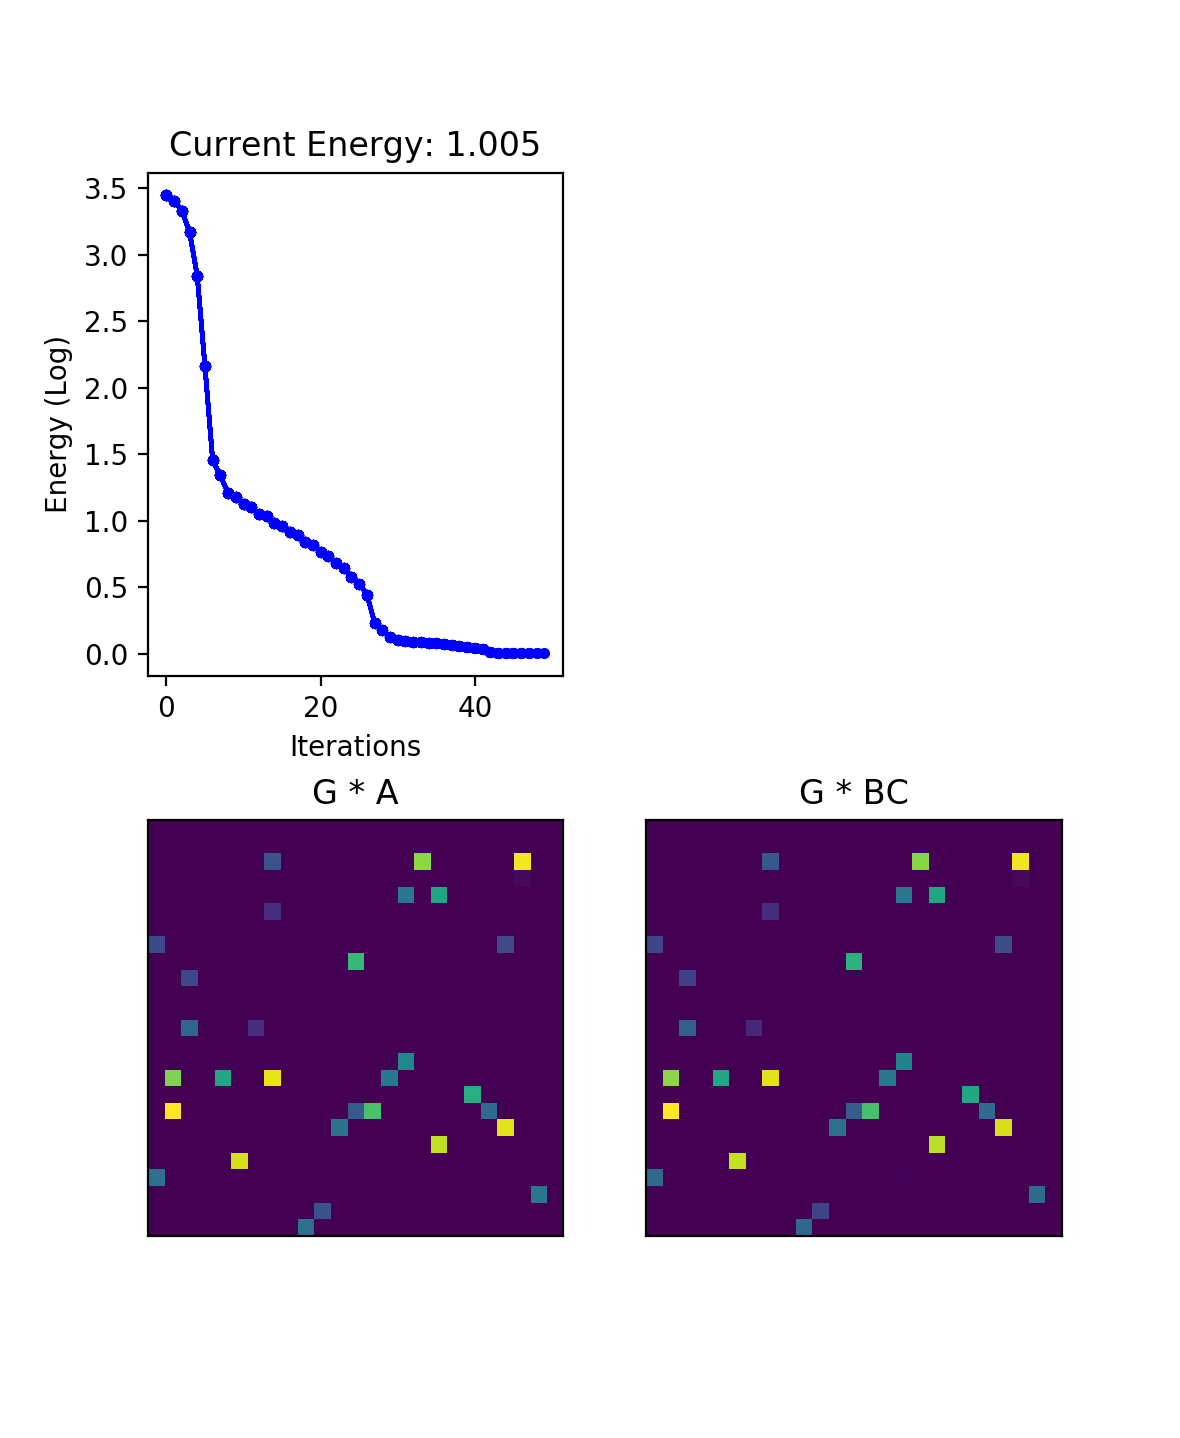
\includegraphics[width=0.5\textwidth]{low_rank_tr.png}
\caption{Results of trust region.}
\end{figure}

\section{Trust Region Conditions with Arbitrary Norm}

Let $B$ be symmetric, $A$ be positive semidefinite. \\

For $p^*$ to be an optimal solution to the following problem
\begin{align*}
\argmin_p & \quad g^\intercal p + \frac{1}{2} p^\intercal B p \\
\text{subject to} & \quad \frac{1}{2} p^\intercal A p \leq \Delta^2
\end{align*}

we have three necessary and sufficient conditions.
\begin{enumerate}
\item $(B + \lambda A) p = -g$
\item $\exists\ \lambda \geq 0$ such that $\lambda (\frac{1}{2} p^\intercal A p - \Delta^2) = 0$
\item $B + \lambda A$ is symmetric positive semidefinite
\end{enumerate}

\begin{lemma} Let $\hat m(p)$ be the following
\begin{align*}
\argmin_p p^\intercal g + \frac{1}{2} p^\intercal B p
\end{align*}

where $B$ is positive semidefinite. \\

Then $\hat m$ attains a minimum if and only if B is positive semi-definite and $g \in Range(B)$. \\

Stated without proof (formal proof in lecture notes). \\

\end{lemma}

\begin{proof} $\impliedby$ \\

We want to show that if $\bar p$ satisfies conditions $1, 2, 3$, then $\bar p = p^\star$. \\

Consider a similar problem.
\begin{align*}
\hat m(p) &= p^\intercal g + \frac{1}{2} p^\intercal (B + \lambda A) p \\
&= m(p) + \frac{1}{2} \lambda p^\intercal A p
\end{align*}

By Lemma 3.1, we know that $\bar p$ is the minimizer to $\hat m$, that is, $\hat m(\bar p) \leq \hat m(p)\ \forall\ p$. 
\begin{align*}
\hat m(\hat p) &\leq \hat m(p) \\
m(\hat p) + \frac{\lambda}{2} \hat p^\intercal A \hat p &\leq m(p) + \frac{\lambda}{2} p^\intercal A p \\
m(\hat p) &\leq m(p) + \frac{\lambda}{2} p^\intercal A p - \frac{\lambda}{2} \hat p^\intercal A \hat p  \\
&= m(p) + \frac{\lambda}{2} p^\intercal A p - \frac{\lambda}{2} \hat p^\intercal A \hat p  + \lambda \Big(\frac{1}{2} \hat p^\intercal A \hat p - \Delta^2 \Big) && \text{By 2.} \\
&= m(p) + \lambda \Big( p^\intercal A p - \Delta^2 \Big) \\
&\leq m(p) && \text{Since $\frac{1}{2} p^\intercal A p \leq \Delta^2$ and $\lambda \geq 0$.}
\end{align*}

We can see that $\bar p$ is the minimizer to $m$.

\end{proof}

\begin{proof} $\implies$ \\

Consider the unconstrained formulation of $m$ (Lagrangian) as
\begin{align*}
\argmin_{p, \lambda \geq 0} \quad p^\intercal g + \frac{1}{2} p^\intercal B p + \lambda \Big( \frac{1}{2} p^\intercal A p - \Delta^2 \Big)
\end{align*}

$p^*$ will lie at a stationary point of the Lagrangian. Taking the gradient with respect to $p$ and setting it to $0$, we have $(B + \lambda A) p = -g$. So we can see $(1)$ is true. \\

Similarly, at a stationary point of the Lagrangian, either $\lambda = 0$, or $\frac{1}{2} p^\intercal A p - \Delta^2 = 0$. Combining these two facts, we have $(2)$. \\

Now we have to consider two cases. \\

Case 1: $\frac{1}{2} p^\intercal A p < \Delta^2$, and $\lambda = 0$. \\

For this, we are on the interior and this turns into unconstrained optimization. We need to show $B + \lambda A$ is positive semi-definite. If $p^*$ is a minimizer, then $B$ is positive semi-definite, by Lemma 3.1, and $B + \lambda A = B$, since in this case $\lambda = 0$. \\

Case 2: $\frac{1}{2} p^\intercal A p = \Delta^2$, and $\lambda > 0$.
\begin{align*}
m(p^*) &\leq m(p) \\
g^\intercal p^* + \frac{1}{2} p^{*^\intercal} B p^* &\leq  g^\intercal p + \frac{1}{2} p^\intercal B p \\
g^\intercal (p^* - p) &\leq \frac{1}{2} p^\intercal B p - \frac{1}{2} p^{*^\intercal} B p^* \\
-p^{*^\intercal} (B + \lambda A)^\intercal (p^* - p) &\leq \frac{1}{2} p^\intercal B p - \frac{1}{2} p^{*^\intercal} B p^* \\
(p - p^*)^\intercal (B + \lambda A) p^* &\leq \frac{1}{2} p^\intercal B p - \frac{1}{2} p^{*^\intercal} B p^* \\
(p - p^*)^\intercal (B + \lambda A) p^* &\leq \frac{1}{2} p^\intercal B p - \frac{1}{2} p^{*^\intercal} B p^* + \frac{\lambda}{2} p^\intercal A p - \frac{\lambda}{2} p^{*^\intercal} A p^* && \text{Since $\frac{1}{2} p^\intercal A p = \frac{1}{2} p^{*^\intercal} A p = \Delta^2$} \\
(p - p^*)^\intercal (B + \lambda A) p^* &\leq \frac{1}{2} p^\intercal (B + \lambda A) p - \frac{1}{2} p^{*^\intercal} (B + \lambda A) p^* \\
0 &\leq \frac{1}{2} p^\intercal (B + \lambda A) p - p^\intercal (B + \lambda A) p^* + \frac{1}{2} p^{*^\intercal} (B + \lambda A) p^* \\
0 &\leq \frac{1}{2} (p - p^*)^\intercal (B + \lambda A) (p - p^*)
\end{align*}

Finally, we must show that $p - p^*$ is dense, that is, $\forall\ u \in \mathbb{R}^n$, we can find $p - p^* = \alpha u$ such that $\frac{1}{2} p^\intercal A p = \Delta^2$. This is equivalent to showing there exists an $\alpha$ such that $\frac{1}{2} (\alpha u + p^*)^\intercal A (\alpha u + p^*) = \Delta^2$.
\begin{align*}
\frac{1}{2} (\alpha u + p^*)^\intercal A (\alpha u + p^*) &= \Delta^2 \\
\frac{1}{2} \alpha^2 u^\intercal A u + \alpha u^\intercal A p^* + \frac{1}{2} p^{*^\intercal} A p^* &= \Delta^2 \\
\frac{1}{2} \alpha^2 u^\intercal A u + \alpha u^\intercal A p^* &= 0 \\
\frac{1}{2} \alpha u^\intercal A u + u^\intercal A p^* &= 0
\end{align*}

We need to show this term is $0$ by picking $\alpha$, and now we have three subcases, depending on properties of $u$. \\

Subcase 1: $u \in Null(A)$. \\

Clearly the term is $0$, since $Au = 0$ by definition. So all values of $\alpha$ satisfy this. \\

Subcase 2: $u^\intercal A p^* \neq 0$. \\

We can simply solve $\alpha = \frac{-2 u^\intercal A p^*}{u^\intercal A u}$. \\

Subcase 3: $u^\intercal A p^* = 0$. \\

We need to show that if this is the case, that $u^\intercal (B + \lambda A) u \geq 0$. Since the space is continuous, for any $u$, we can define a function $\hat u(\epsilon) = u + \epsilon p^*$. \\

From the two subcases above, we know $\lim_{\epsilon \rightarrow 0^-} \hat u(\epsilon)^\intercal (B + \lambda A) \hat u(\epsilon) = \lim_{\epsilon \rightarrow 0^+} \hat u(\epsilon)^\intercal (B + \lambda A) \hat u(\epsilon) \geq 0$. By continuity, we have our result that $u^\intercal (B + \lambda A) u \geq 0$.

\end{proof}

\end{document}
